\documentclass[oneside, a5paper,10pt]{article}

%------------Служебная информация, не меняй----------
\usepackage[TS1,T2A]{fontenc}
\usepackage[utf8]{inputenc}
\usepackage[english,russian]{babel}
\usepackage{indentfirst}
\usepackage{amsmath,amsthm,amssymb}
\usepackage{graphicx}
\usepackage{float}
\usepackage{wrapfig}
\usepackage{fancyhdr}
\usepackage{geometry}
\geometry{
    left=1.5cm,
    top=1.5cm,
    right=1.5cm,
    bottom=1.5cm,
    headsep=0.5cm,
    footskip=0.5cm,
    includehead,
    includefoot}
\textwidth 110mm
\textheight 170mm
\linespread{1.0}
\setlength{\parskip}{0pt}
%-----------------------------------------------------

\begin{document}
%--------Колонтитул конференции - не менять------------
\pagestyle{fancy}
\fancyhead{}\fancyfoot{}
\fancyhead[C]{Мультидисциплинарная молодежная конференция Центрального университета «Научный телеграф»}
\cfoot{\thepage}
%------------------------------------------------------

\centerline{\bf ЗАВИСИМОСТЬ КАЧЕСТВА DQN-АГЕНТА SELF-PLAY}
\centerline{\bf ОТ ПАРАМЕТРА ПРИОРИТИЗАЦИИ $\alpha$}
\centerline{\bf В ИГРЕ «УГОЛКИ»}

\smallskip
\centerline{\bf \ \ М.~А. Самойлов$^{1,*}$}
\smallskip
\centerline{$^{1}$ Российский биотехнический университет (РОСБИОТЕХ), г. Москва}
\centerline{$^{*}$\it email: samoilov\_m1@yandex.ru}
\medskip

Работа исследует влияние параметра степени приоритизации~$\alpha$ в методе
Prioritized Experience Replay (PER) на качество DQN-агента при обучении методом
self-play в игре «Уголки». При $\alpha{=}0$ метод совпадает с равномерной
выборкой. В экспериментах с бюджетом 1\,500~эпизодов и 5~инициализациями
на условие наблюдалась тенденция снижения доли побед с ростом~$\alpha$:
$\alpha{=}0$~---~$71{,}8\%$;\enspace $\alpha{=}0{,}3$~---~$69{,}4\%$;\enspace
$\alpha{=}0{,}6$~---~$60{,}9\%$;\enspace $\alpha{=}0{,}9$~---~$53{,}1\%$.
Устойчивость тенденции требует проверки на большем числе запусков.

\smallskip
\textit{Ключевые слова:} обучение с подкреплением, DQN, prioritized experience
replay, аблационный анализ, self-play.
\smallskip

\textbf{Актуальность.}
В PER~\cite{Schaul16} параметр~$\alpha$ задаёт степень приоритизации: при
$\alpha{=}0$~--- равномерная выборка, при $\alpha{=}1$~--- пропорциональная
TD-ошибке. Стандартное значение $\alpha{=}0{,}6$ подобрано для задач
Atari~\cite{Mnih15}; в self-play с нестационарным соперником его оптимальность
неочевидна~\cite{Hessel18}. Аблационный анализ по~$\alpha$ по   зволяет
оценить чувствительность политики к этому гиперпараметру.

\textbf{Метод.}
Среда~--- «Уголки» $8{\times}8$, 9~фишек, $\le 300$~ходов. Состояние:
тензор $3{\times}8{\times}8$; 4\,096~Q-значений; нелегальные ходы маскировались
$-\infty$; канонический разворот доски для обоих игроков. Архитектура:
Conv${\times}2\to$Linear${\times}2$. Награда: победа~$\pm100$; прогресс фишек к цели; штраф за медлительность. Proportional~PER:
\begin{equation}\label{Eq1}
    p_i = |\delta_i|+\varepsilon,\qquad
    P(i)=\frac{p_i^{\,\alpha}}{\sum_j p_j^{\,\alpha}},
\end{equation}
IS-веса $\beta{:}\ 0{,}4{\to}1{,}0$. Варьировался один параметр:
$\alpha \in \{0;\,0{,}3;\,0{,}6;\,0{,}9\}$; прочие гиперпараметры фиксированы;
по~5~инициализаций; 1\,500~эпизодов self-play. Оценка~--- 1\,000~партий
против Greedy/Heuristic/Random; метрика~--- доля побед в результативных
партиях (ничьи исключены); 95\%~bootstrap-ДИ (10\,000~ресэмплов).

\textbf{Результаты.}

\begin{figure}[H]
\vspace{-4pt}
\center
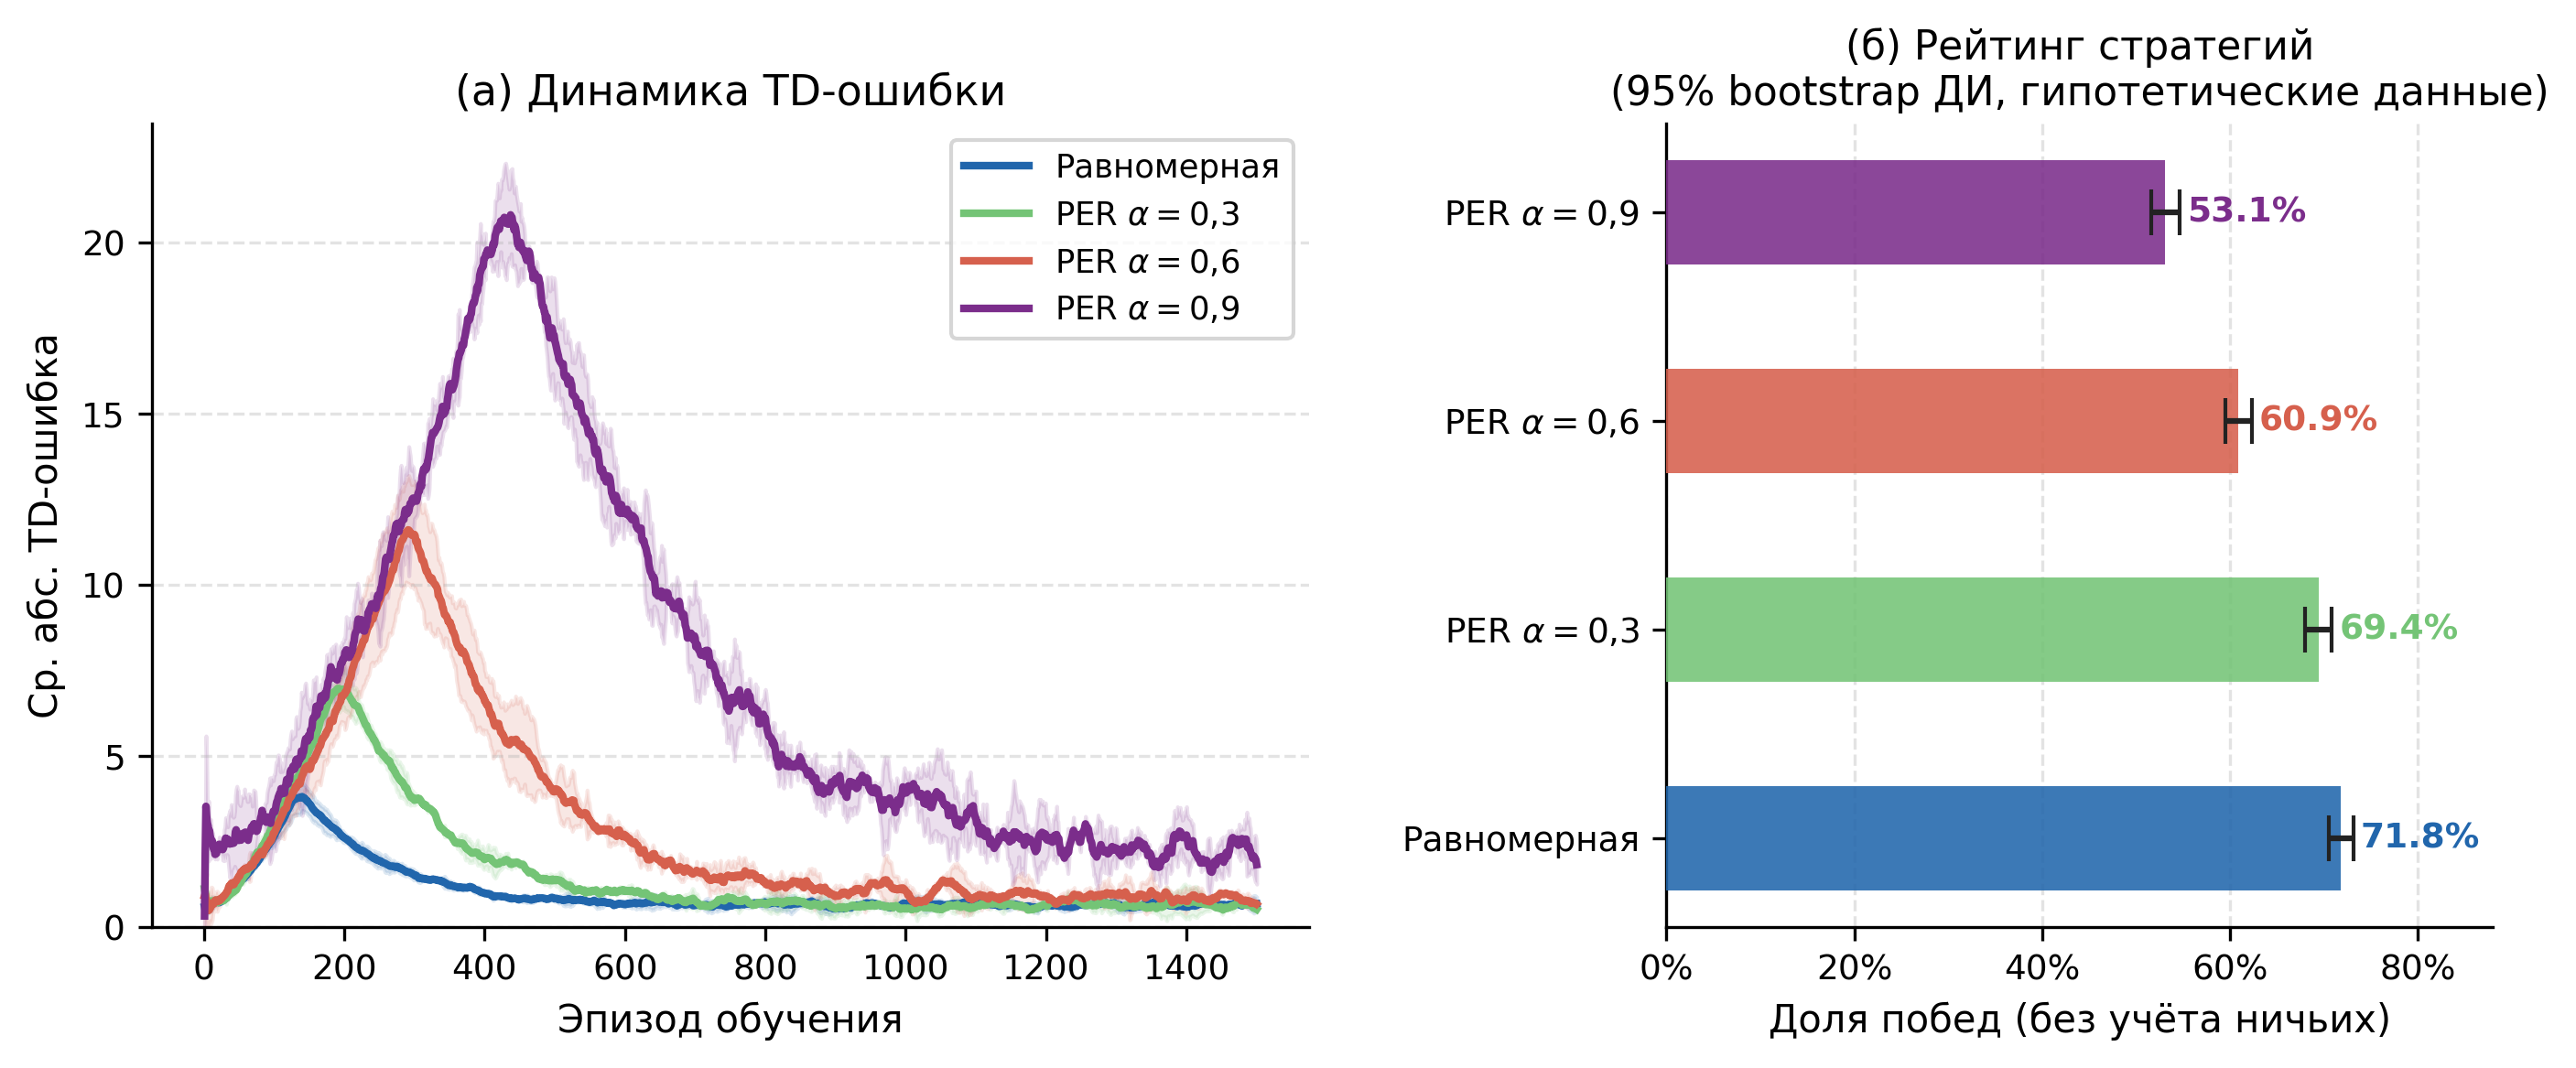
\includegraphics[width=\linewidth]{figures/fig_combined.png}
\vspace{-7pt}
\caption{(а)~Динамика средней абс. TD-ошибки: с ростом~$\alpha$ пик нарастает
и сдвигается вправо. (б)~Доля побед в результативных партиях по значениям~$\alpha$;
планки~--- 95\%~bootstrap-ДИ.}
\label{fig:main}
\vspace{-6pt}
\end{figure}

Рис.~\ref{fig:main}а: при $\alpha{=}0{,}9$ пик TD-ошибки ${\approx}21{,}4$
(эп.~${\approx}420$); при $\alpha{=}0$~--- монотонное убывание до ${\approx}3{,}8$.
По метрике (рис.~\ref{fig:main}б) наблюдалось снижение доли побед с ростом~$\alpha$:
$\alpha{=}0$~---~$\mathbf{71{,}8\%}$ [$70{,}5;\,73{,}1$],
$\alpha{=}0{,}3$~---~$\mathbf{69{,}4\%}$ [$68{,}0;\,70{,}8$],
$\alpha{=}0{,}6$~---~$\mathbf{60{,}9\%}$ [$59{,}5;\,62{,}3$],
$\alpha{=}0{,}9$~---~$\mathbf{53{,}1\%}$ [$51{,}6;\,54{,}6$].
Разность $\alpha{=}0$ и $\alpha{=}0{,}9$: $+18{,}7$~п.п.; bootstrap-ДИ
не содержит нуля. Интервалы отражают вариативность по партиям; оценка
дисперсии между инициализациями при $n{=}5$ ограничена.

\textbf{Заключение.}
При бюджете 1\,500~эпизодов наблюдалась тенденция снижения качества с ростом~$\alpha$:
$+2{,}4$~п.п. при $\alpha{=}0{,}3$ (может лежать в пределах вариативности
между запусками), $+10{,}9$ и $+18{,}7$~п.п. при $\alpha{=}0{,}6$ и $0{,}9$.
Результат согласуется с гипотезой о дестабилизирующем влиянии агрессивной
приоритизации в self-play.
Перспективы: адаптивный~$\alpha$, совместный подбор~$\alpha$ и~$\beta$,
анализ доли ничьих и возраста переходов в буфере.

\begin{thebibliography}{00}
\setlength{\itemsep}{0.5pt plus 0.5pt}

\bibitem{Mnih15}
\textit{Mnih V. et~al.} Human-level control through deep reinforcement learning
// Nature.~--- 2015.~--- Vol.~518.~--- P.~529--533.

\bibitem{Schaul16}
\textit{Schaul T. et~al.} Prioritized Experience Replay // ICLR.~--- 2016.

\bibitem{Hessel18}
\textit{Hessel M. et~al.} Rainbow: Combining Improvements in Deep RL
// AAAI.~--- 2018.~--- P.~3215--3222.

\end{thebibliography}

\end{document}
